\chapter{A Plagiarism Primer}\label{chap:plagOverview}

Here we will introduce you to the topics we encountered and researched in the beginning of the Unplagged project.

\section{Plagiarism definition}

% Das können wir meiner Meinung nach so nicht lassen, wir können doch nicht die Definition von Plagiat abschreiben..

You will probably have learned as a child, that stealing material goods is something that will get you arrested sooner or
later. Somehow many people make a huge difference when it comes to intellectual property, maybe due to the fact that 
stealing ideas or texts is much easier to do and much harder to catch.

Nonetheless, this is something that would fall under copyright laws and is also a crime, which could get prosecuted.

Here is what \citet{PlagiarismDotOrg} thinks about plagiarism:

\begin{quote}\enquote{
Many people think of plagiarism as copying another's work, or borrowing someone else's original ideas. But terms like 
\enquote{copying} and \enquote{borrowing} can disguise the seriousness of the offense: [...] In other words, plagiarism 
is an act of fraud. It involves both stealing someone else's work and lying about it afterward.
}
\end{quote}

The Community Standard for Undergraduates of the \citet{DukeSite} University  shows examples for the difference between intentional and unintentional Plagiarism:

\textbf{Intentional Plagiarism}


\begin{itemize}
\item Purchasing a pre-written paper (either by mail or electronically).
\item    Letting someone else write part or all of a paper for you.
\item    Paying someone else to write part or all of a paper for you.
\item    Submitting as your own someone else's unpublished work (including a computer program or algorithm), either with or without permission.
\item    Submitting as your own, work done jointly by a group in which you may have participated.
\item    Submitting work done by you, but for another class or another purpose without documenting that it was previously used.
\item    Creating phony citations.
\end{itemize}

\textbf{Unintentional Plagiarism}
\begin{itemize}
\item Failure to cite a source that is not common knowledge.
\item Failure to "quote" or block quote author's exact words, even if documented.
\item Failure to put a paraphrase in your own words, even if documented.
\item Failure to put a summary in your own words, even if documented.
\item Failure to be loyal to a source.
\end{itemize}




	
	
\section{Basic Classification of Plagiarisms}

In this part, we will try to cover common classifications of plagiarism, but at first we want to figure out the purpose of 
the classification. 

There are many reasons explaining why people plagiarize. Generally those include, that they didn't have the time,
energy or the ability to do the work by themselves or that they try to steal other’s work on purpose with the hope that 
others
will not recognize it. This kind of plagiarism is done intentionally and named \textit{deliberate 
plagiarism}\citep{UEfAP}.

Another kind is \textit{accidental plagiarism}. This occurs when texts from some sources are copied or rephrased, but no 
reference is given. The reason is that the writer didn't know that it is a plagiarism because of \enquote{carelessness or  
lack of skill}\citep{UEfAP} while writing.

Anyway, it is important to know, that working with the source carelessly may cause plagiarism. Classification 
of plagiarism is also a good way to help distinguish typical types of plagiarism, so that people are aware and able 
to reference the sources carefully and to avoid plagiarizing.

Classification of plagiarism is also good for professors or the plagiarism detection community such as VroniPlag, because
it gives them a common terminology, which enables them to communicate faster and more efficiently. 
It also helps them to realize what category and how many percent the text is plagiarized 
if there is any suspicion, so that statistical data can be created.

% I don't understand this sentence at all..
%So the classification is about the way to detect plagiarism while conducting a citation. 
But what is a citation, and 
what kinds of citation are there? Understanding of citations and the way to cite is an important thing in order to 
avoid and detect plagiarism.

\subsection{Definition of Citation}

\begin{quote}\enquote{A citation is a credit or reference to another document or source}\\ \citep{wiki:Citation}\end{quote}

According to this definition, citation is your reference to a source of information, which was generated by someone 
and should be indicated properly when this source is used in your work.

Based on \citet{Wiredprof2010}, there are 3 forms of citation:

\begin{description}
\item[Direct quotation:] \hfill \\
That is an exact word-to-word copy from one \textit{source}. In this case, in order to cite you have to mark 
the text with quotation marks and indicate a  parenthetical referencing, which includes the \textit{book’s name and the page 
number} where you found the source.
\item[Paraphrase:] \hfill \\
That is your own explanation of someones idea. Many people think it is not a plagiarism because the text 
is written with your own words. But it is still a plagiarism because basically that is not your idea or your opinion, 
but the author’s himself. In this case of citation, some keywords are still kept in the work. Therefore the 
parenthetical reference must be given.
\item[Summary:] \hfill \\
That is the same as paraphrase, but this kind of citation is likely a \textit{summary} of the text. In this case you 
have to give the parenthetical referencing as well.
\end{description}

Now we can see that citation has a lot of forms. You are free to use the source but you have to make sure to cite 
sources properly 
or you are applying a plagiarism.

After understanding what citation is and its form, now we can try to classify the plagiarism. The criteria which we 
choose for classification are based on the VroniPlag’s plagiarism categories, because Unplagged is mostly based 
on the workflow of the VroniPlag community. 

By VroniPlag, it does not matter what citation standard system is used in the work, but it is important to know how the 
citation is documented and if the reference is given properly.

\subsubsection{VroniPlag’s classification of plagiarism}\label{sec:classification}

According to VroniPlag\citep{} there are the following plagiarism categories. 
The categories are originally written in German, and the translation or the similar category in English is written 
right after the german expression.

\begin{description}
\item[Komplettplagiat/Copy \& Paste\citep{one12}:] \hfill \\
The name of this category already indicates how the text is plagiarized. The 
plagiariser just copies from the source exactly word-by-word and does not leave any proper reference to the source 
intentionally. Some is too lazy so that they just copy existing mistakes, formats etc... without checking, which 
later can become a proof of plagiarism.

The category is differentiated by the way of conducting a citation.
Source is not cited: the original text is completely copied but the source reference is not given intentionally.
Source is cited but not completely: reference is given but not correctly.  

\item[Verschleierung/Paraphrasing\citep{PlagiarismSearch}:]  \hfill \\
The texts from different sources are rephrased and mixed together. The plagiariser tries 
to hide his stealing by changing some word orders, replacing words with synonyms … The source is not given with the hope, 
that the text is considerably generated by the plagiariser himself and therefore the plagiarism will not be detected.

\item[Übersetzungsplagiat/translations\citep{one12}:] \hfill \\
This kind of plagiarism occurs when the sources in foreign languages are translated. 
The plagiariser pretend that this translated text is his own work. Sources are oft not given properly. This is a 
well-liked way in researching because there are many translation tools which can be found easily in Internet such as 
Babelfish, Google Translate … and  it is not easy to detect the plagiarism with existing plagiarism detection tools.

\item[Alibi-Fußnote/The forgotten Footnote\citep{PlagiarismSearch}:] \hfill \\
in this category, the source is cited but the real location of the source is 
hidden.  

\item[Bauernopfer und. Verschärftes Bauernopfer:] \hfill \\
The source reference is embedded in footnote part but it redirects to 
another text part of the source which has no relation with the plagiarized text.
\end{description}

\paragraph{Other categories}


\begin{description}
\item[Halbsatzflickerei/The Labor of Laziness\citep{PlagiarismSearch}:] \hfill \\
The plagiariser takes sentences, or just parts of sentence from different 
sources, tries to reword them and mixes all so that they look fit together. Source reference is not or not correctly 
given.

\item[Shake \& Paste\citep{one12}:] \hfill \\
The sentence or paragraph from one source is mixed with one from another source. This 
plagiarism can be detected by changes of writing styles. Source reference is also not given properly.
\end{description}

\section{How to detect plagiarism}
Plagiarism detection means a lot of effort and hard work, because a lot of documents, books and papers must be found, scanned and compared line for line. Often it is really complicated to find available sources in libraries or scientific database systems and plenty of pages must be copied by hand. 
During the last ten years a lot of software companies came into market to automatize this process and developed algorithms to find plagiarisms automatically. These systems are called "Plagiarism detection systems (PDS) ". 
There are two different approaches for plagiarism detection systems to identify plagiarism in text documents:
\begin{enumerate}
\item \textbf{Corpus based analysis}\\
means to "compare suspicious documents against a set of potential original documents" \citet{PAN:2007} to find similar text passages.
\item \textbf{Intrinsic analysis}\\
"identifies potentially plagiarized passages by analyzing the suspicious document with respekt to changes in writing style". \citep{PAN:2007}
\end{enumerate}
These computer assisted detection systems alone are not appropriate to find all plagiarisms without human judgement.  

 \begin{figure}[!h]
  \centering
  \fbox{
    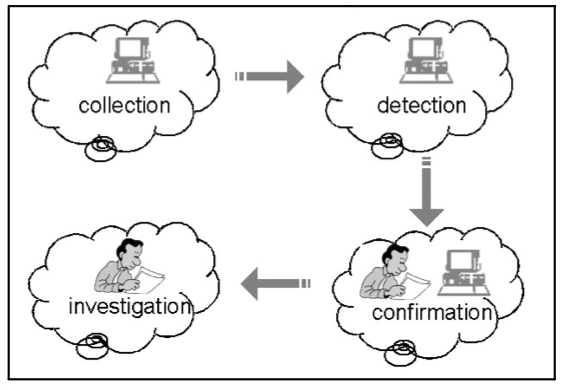
\includegraphics[width=0.97\textwidth]{images/4-steps.png}
  }
  \caption{4-stage plagiarism detection process}
  \label{fig:4-stage plagiarism detection process}
\end{figure}

We found out that the most practical way is to combine both approaches - the first step is to use the computer-based detection to find similarities between the suspicious documents and the original papers. The second step is to examine the results, validate them and continue the search in a deeper level.\citep{PI:2001} (see figure \ref{fig:4-stage plagiarism detection process}) 



\section{Commercial software systems} 

 
 \begin{figure}[!h]
  \centering
  \fbox{
    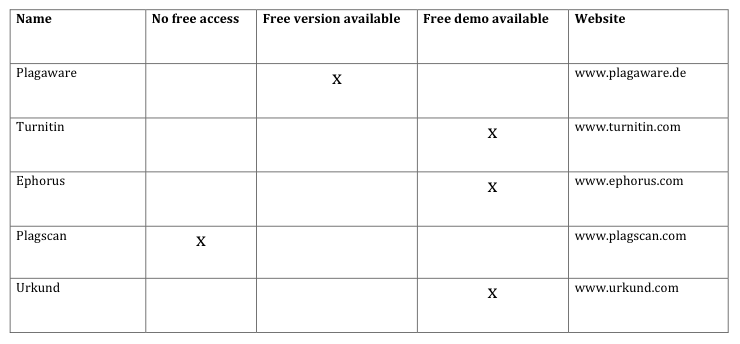
\includegraphics[width=0.97\textwidth]{images/software_systems/overview.png}
  }
  \caption{Overview of Commercial Detection Systems}
  \label{fig:overview_systems}
\end{figure}



Several computer companies developed commercial software systems to facilitate the detection of plagiarism. They offer different terms of pricing and online as a service or offline programs. 
The software system compare digital content from the internet or different types of databases. 
They seek for similarities, report suspicious parts and try to answer the question if the present text is a plagiarism or not.

This chapter covers parts of the results of the big "Plagiarism Detection System Test 2010". 
The following benchmarking was done by Prof. Debora Weber-Wulff at the University of Applied Sciences HTW Berlin and her plagiarism team in 2010. \citep{PlagiatTeam} 
The entire benchmarking includes 26 of the 47 available systems on the market and gives an overview of the strengths and weaknesses of these systems in finding plagiarism.

We used the top 5 "partially useful" software systems in this  benchmarking to overview the market and find the best usable features for our own system to simplify the daily work of plagiarism finders. 
\citep{PlagiatTeam} 






\newpage



\subsection{PlagAware} 
 \begin{figure}[!h]
  \centering
  \fbox{
    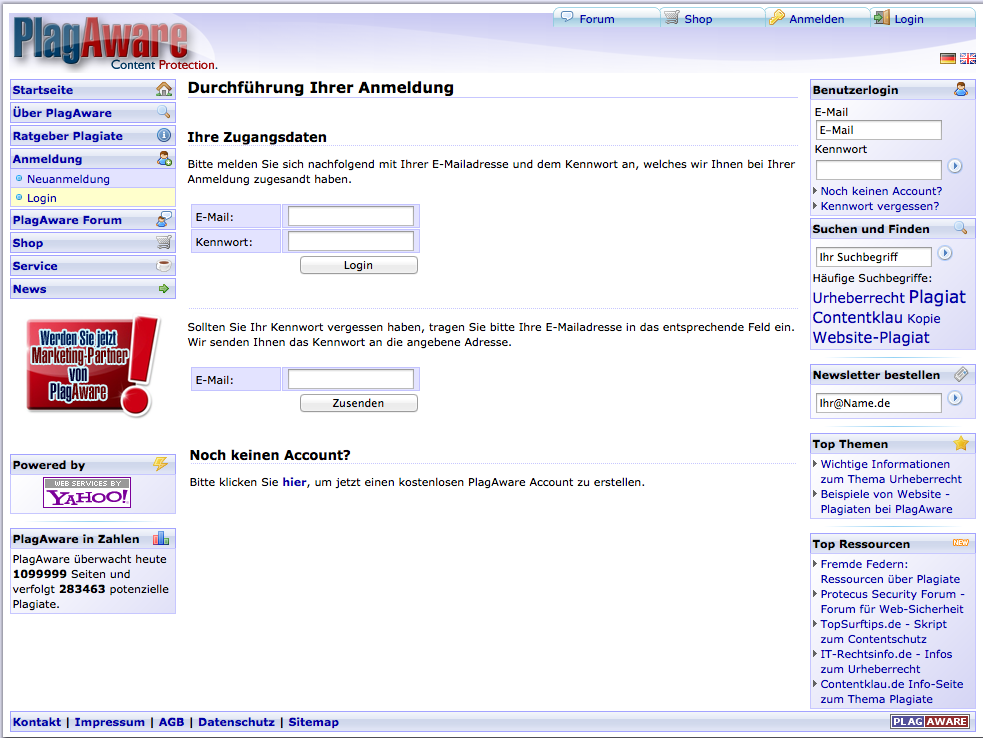
\includegraphics[width=0.97\textwidth]{images/software_systems/plagaware_1.png}
  }
  \caption{Plagaware Website}
  \label{fig:plagawareWebsite}
\end{figure}


\textbf{Plagaware Business Promotion}
\begin{quote}
"PlagAware is an online-service, which offers services around the topics Searching, finding, analysing and tracing of plagiarisms. The central element of PlagAware is a search engine, which is specialised in detecting identical contents of given texts. Contrary to the plagiarism scanning with classical search engines, the places of finding are not directly transferred to the user, but analysed on the rate and the type of analogy, before a message to the user is written. By this the differing result reports of PlagAware allow to recognise very fast the percentage and the distribution of the copied text contents, thus permitting an efficient and secure rating of a possible plagiarism."  
\end{quote}\citep{PlagawareTest}


PlagAware is software company from Ulm in Germany. The website is online for nearly 5 years and is the top-ranked system in the HTW "Plagiarism Detection System Test" 2010, but in fact it still detect only 61,11\% of the plagiarism cases. 
Although PlagAware "produces excellent documentation of the plagiarism found, highlighting the commonalities in a side-by-side presentation. However, its usefulness at university is limited, as each file must be uploaded individually - no ZIP file or student-submission is possible. The system was not designed to be used in a university setting, but rather to find plagiarisms of online texts, which is important for sites trying to optimize their search machine ranking, as plagiarism will contribute to downranking." \citep{PlagawareTest}

Figure Overview shows an overview of all fragments and the results of the plagiarism detection. In figure Side-by-side shows a nice side-by-side fragment view, where all found plagiarisms are shown with different colors. Anomalies in the text are highlighted and the barcode-view is available.
 
 \begin{figure}[!h]
  \centering
  \fbox{
    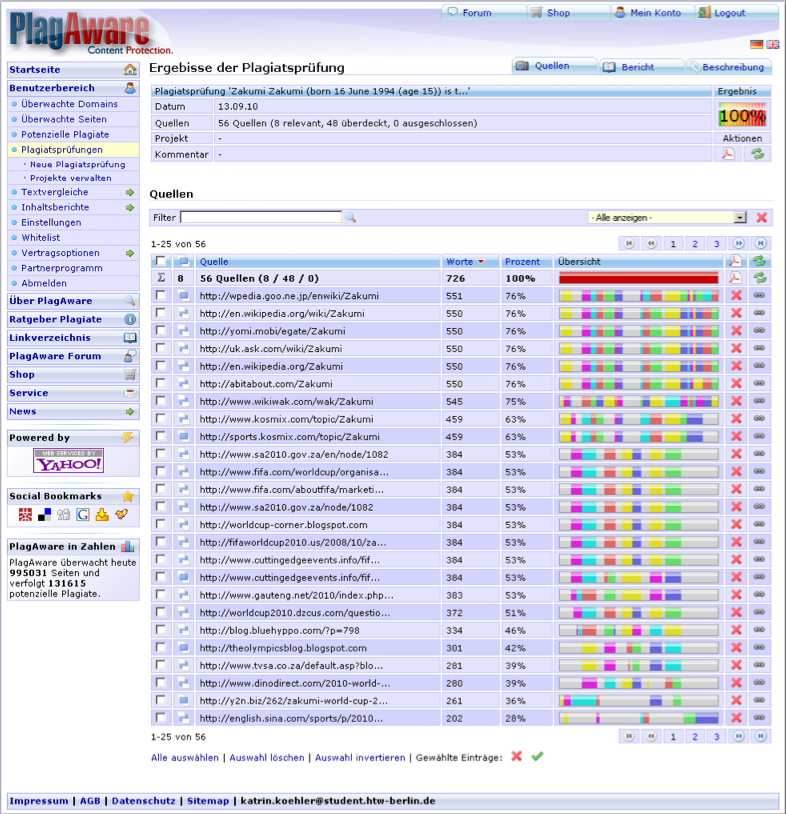
\includegraphics[width=0.97\textwidth]{images/software_systems/plagaware_2.png}
  }
  \caption{Plagaware overview}
  \label{fig:plagawareoverview}
\end{figure}


 \begin{figure}[!h]
  \centering
  \fbox{
    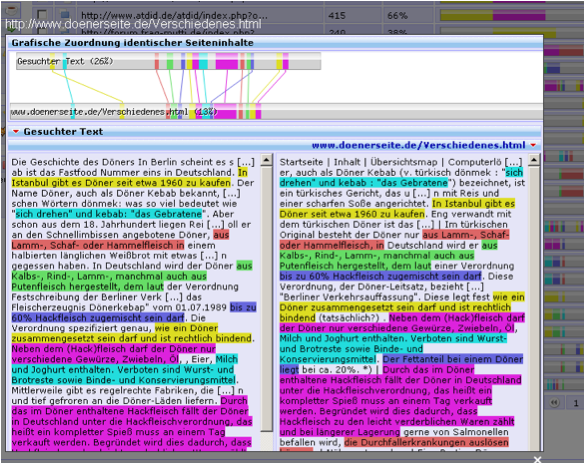
\includegraphics[width=0.97\textwidth]{images/software_systems/plagaware_3.png}
  }
  \caption{Plagaware side-by-side view}
  \label{fig:plagaware_side_by_side}
\end{figure}


\newpage
\subsection*{PlagAware Costs}
PlagAware has four different payment-models:
\begin{enumerate}
\item \textbf{Free}\\
30 scans/month for free. Every additional scan costs 3,0 ct. 
\item \textbf{Light}\\
EUR 2,99/month. 150 scans/month included. Every additional scan costs 2,0 ct. Mininum term of 6 month.
\item \textbf{Standard}\\
EUR 7,49/month. 500 scans/month included. Every additional scan costs 1,5 ct. Mininum term of 6 month.
\item \textbf{Premium}\\
EUR 14,99/month. 1500 scans/month included. Every additional scan costs 1ct. Mininum term of 6 month.
\end{enumerate}\citep{PlagawareTest}



\newpage
\subsubsection{Turnitin} 
 \begin{figure}[!h]
  \centering
  \fbox{
    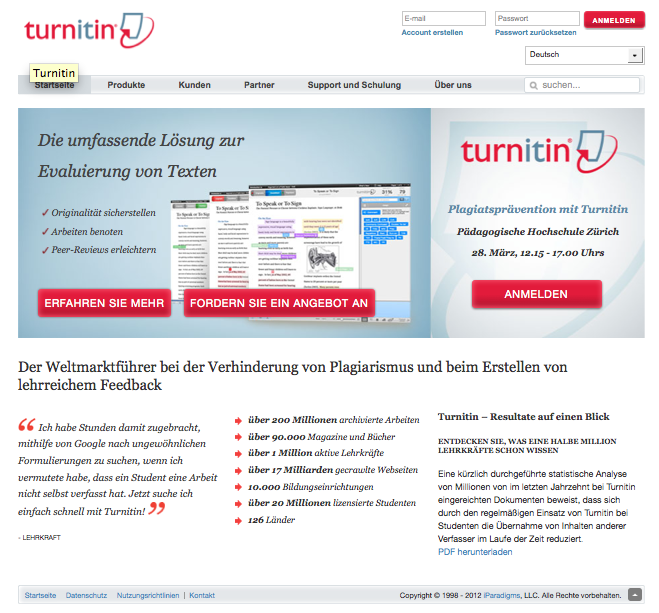
\includegraphics[width=0.97\textwidth]{images/software_systems/turnitin_1.png}
  }
  \caption{Turnitin Website}
  \label{fig:Turnitin Website}
\end{figure}

\textbf{Business Promotion}
\begin{quote}
"Our award-winning solution discourages plagiarism and facilitates rich, meaningful feedback that improves writing skills, promotes critical thinking, and streamlines grading."
\end{quote}
\enquote{Turnitin}\citep{Turnitin Business Promotion}\href{http://www.turnitin.com}{Turnitin}


Turnitin is a product by a company called iParadigms. It is a well-known US plagiarism software system and one of the most used plagiarism detection systems in the education sector. The website is online for nearly 13 years and the system is at the second position in the HTW "Plagiarism Detection System Test" 2010.  

The best results can be achieved with material which is already in the database. 

In the past the had a lot of problems to deal with umlauts, and having a complex setup. They improved a lot of parts especially the german translation. Still a big problem for european countries is the copyright policy of Turnitin. They still storing copies of user material in their database without a permission. \citep{TurnitinTest}

 \begin{figure}[!h]
  \centering
  \fbox{
    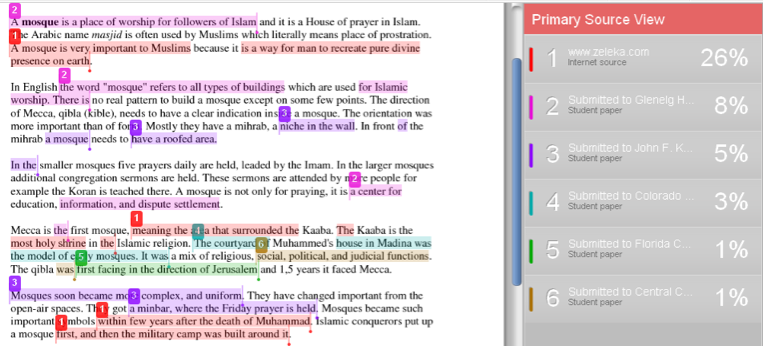
\includegraphics[width=0.97\textwidth]{images/software_systems/turnitin_3.png}
  }
  \caption{Turnitin - A lot of little matches can't be found, if the sensibility has not been raised.}
  \label{fig:Turnitin overview}
\end{figure}
 
In 2008 the system was placed at the 13th position. The reason of this change is that the others systems have gotten worse. Turnitin has still problems of flagging spam sites especially when this sites are not safe for work (e.g. site with pornography content) (see \ref{fig:TurnitinSpamExample}). This is a problem when students uses school or university computers.
On the other hand the search algorithm of Turnitin is storing sites in their database although they are still not exist.\citep{TurnitinTest}


\subsection*{Costs}
There are different license models for the education sector and the cost depends on the amount of users . 

 \begin{figure}[!h]
  \centering
  \fbox{
    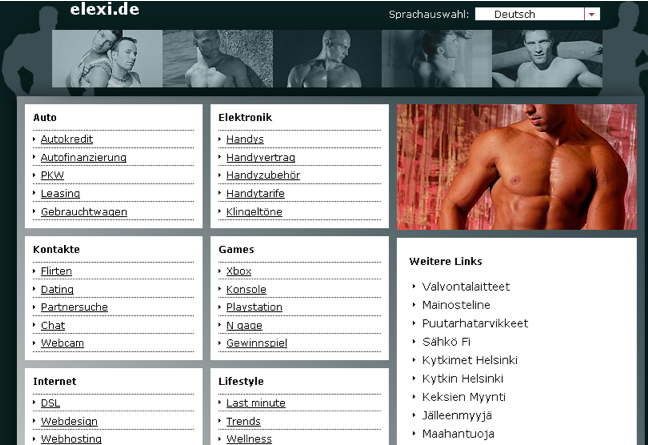
\includegraphics[width=0.97\textwidth]{images/software_systems/turnitin_4.png}
  }
  \caption{Turnitin - A lot of spam-sites are reported. Not all sufficient to use at work. This is one of the harmless examples.}
  \label{fig:TurnitinSpamExample}
\end{figure}






\newpage

\subsection{Ephorus}

 \begin{figure}[!h]
  \centering
  \fbox{
    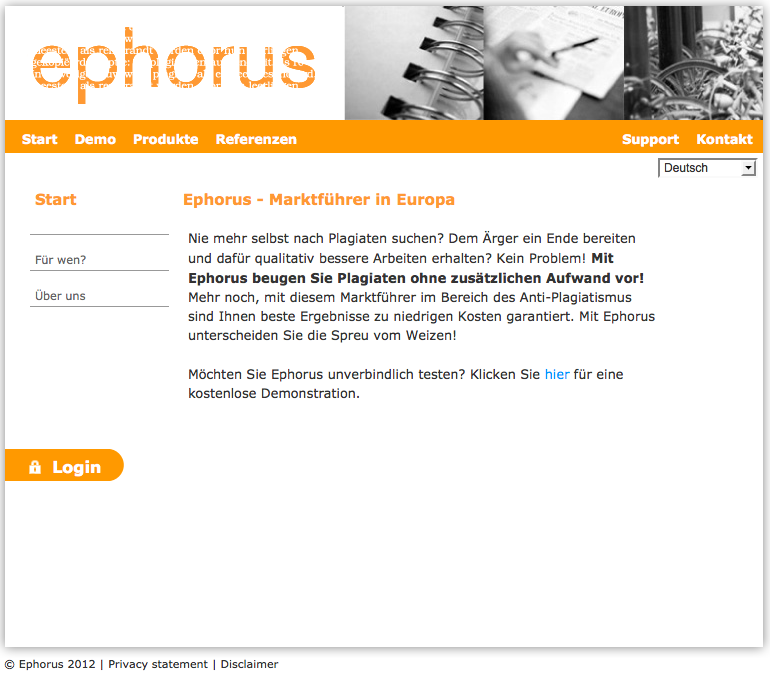
\includegraphics[width=0.97\textwidth]{images/software_systems/euphorus_1.png}
  }
  \caption{Ephorus Website}
  \label{fig:plagawareWebsite}
\end{figure}

\textbf{Business Promotion}
\begin{quote}
"Never search for plagiarism yourself again? An end to all irritations and qualitatively better papers? No problem. With Ephorus, you can prevent plagiarism with no extra effort. Moreover, with this anti-plagiarism market leader, you will be assured of the best service and the lowest prices. With Ephorus, teaching will be fun again! Would you like to try out Ephorus?
\end{quote}
\citep{EphorusTest}

The third position in the HTW "Plagiarism Detection System Test" 2010 is Euphorus. It's a plagiarism detection system from the netherlands and the website is online for nearly 8 years.
2007 it took the first place in the test, 2008 it was only position 8. Now they redisigned and reorganized the system and old problems were solved. The usability of reports and the whole handling of the system very good. (figure: report)But their still problems with umlauts and the european copyright problematic like in Turnitin. (figure: umlauts)


 \begin{figure}[!h]
  \centering
  \fbox{
    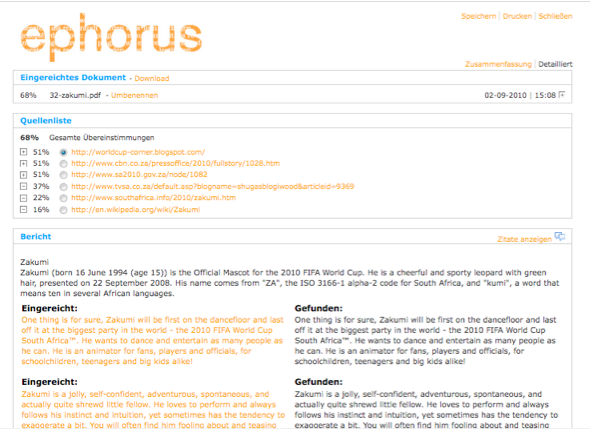
\includegraphics[width=0.97\textwidth]{images/software_systems/euphorus_3.png}
  }
  \caption{Ephorus report - gives a great overview of the results}
  \label{fig:Ephorus_report}
\end{figure}




\subsection*{Ephorus costs}
Not stated.

 \begin{figure}[!h]
  \centering
  \fbox{
    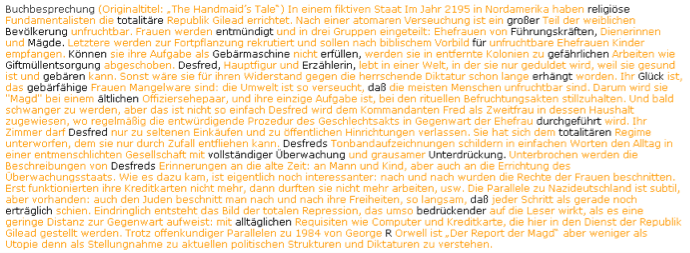
\includegraphics[width=0.97\textwidth]{images/software_systems/euphorus_5.png}
  }
  \caption{Ephorus Problem with umlauts}
  \label{fig:Euphorus_umlauts}
\end{figure}













\newpage
\subsection{PlagScan} 

 \begin{figure}[!h]
  \centering
  \fbox{
    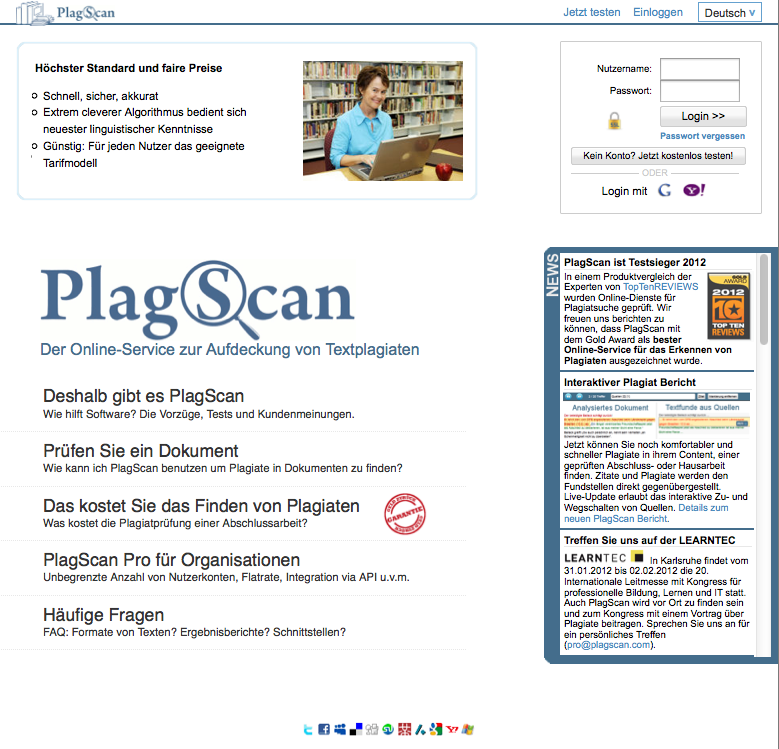
\includegraphics[width=0.97\textwidth]{images/software_systems/plagscan_1.png}
  }
  \caption{Plagscan Website}
  \label{fig:plagawareWebsite}
\end{figure}


\textbf{Business Promotion}
\begin{quote}
\textbf{PlagScan stands for professionalism}
\begin{itemize}
\item All documents are treated 100\% confidential
\item    You control whether your document is checked against others, or not
\item    Integration via API in your existing CMS or learning management system possible
\end{itemize}
\textbf{Plagiarism check as easy as pie: PlagScan}
\begin{itemize}
\item    Annotations directly in the document, check without additional work
\item    No installation - complete functionality in every browser
 \item   All popular formats can be processed
\end{itemize}
\textbf{Save time with PlagScan}
\begin{itemize}
\item    Check several documents in parallel.
\item    Fully automated document analysis.
 \item   No use of your resources, all computation is carried out on our servers.
\end{itemize}

\end{quote}
\enquote{Plagscan Business Promotion}\citep{PlagscanTest}

Plagscan is a software company from Mainz, Germany. It placed at position number 4 in the HTW "Plagiarism Detection System Test" 2010. The website is online for 3 years and in the preview check 2008 it came to the 10th position.
As a user you have to buy "Plag Points" (PP). One test costs 1 PP per 100 words. 
The administrator sets up users and assigns them points for use.
There are three different kinds of reports - a list of possible sources with links to click on, the submitted document with the suspicious areas linked to a possible source, and a docx file with the sources in comments.
There's no side-by-side presentation, so it's not possible to compare the fragments.
Although there are still problems, PlagScan was first place in usability, but only 8th place in overall effectiveness with only 60\% of the points awarded for finding plagiarisms.\citep{PlagscanTest}


 \begin{figure}[!h]
  \centering
  \fbox{
    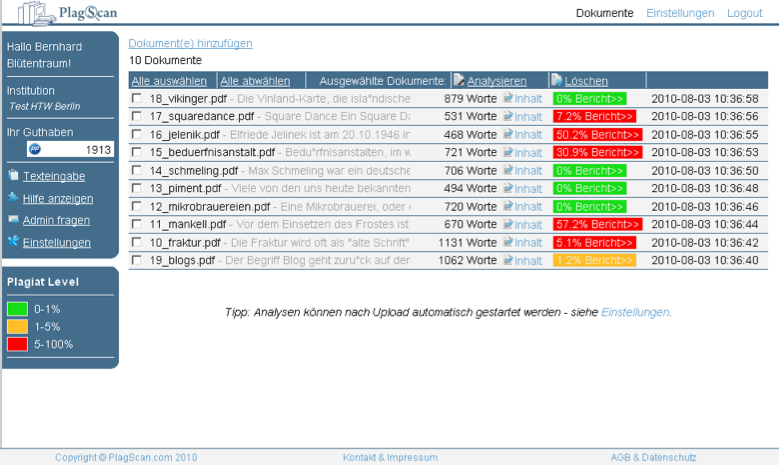
\includegraphics[width=0.97\textwidth]{images/software_systems/plagscan_2.png}
  }
  \caption{Plagscan report is clear and tidy.}
  \label{fig:plagaware report}
\end{figure}


 \begin{figure}[!h]
  \centering
  \fbox{
    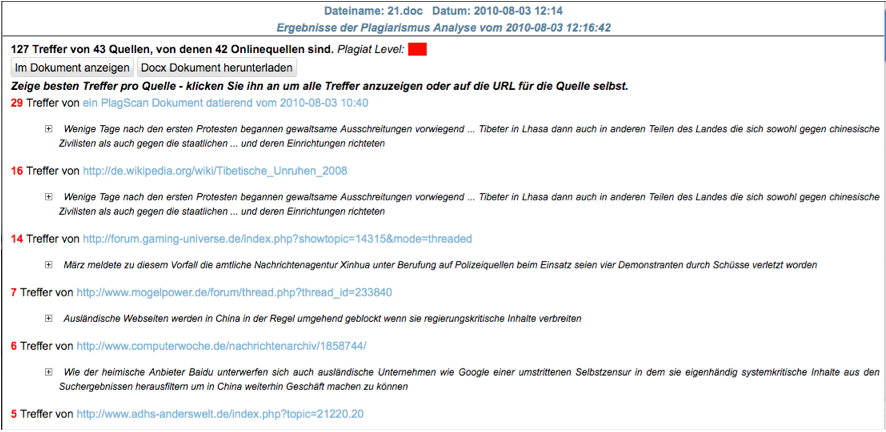
\includegraphics[width=0.97\textwidth]{images/software_systems/plagscan_3.png}
  }
  \caption{Plagscan reports are not self-explanatory.}
  \label{fig:plagaware report 2}
\end{figure}

\subsubsection{Plagscan costs}
PlagScan has four different payment-models without a contract:
\begin{enumerate}
\item \textbf{9 Euro}\\
500 Plagpoint - 50.000 words - 200 Sites. 
\item \textbf{19 Euro}\\
1.250 Plagpoints - 125.000 words - 500 Sites. 
\item \textbf{29 Euro}\\
2.000 Plagpoints - 200.000 words - 800 Sites. .
\item \textbf{69 Euro}\\
5.000 Plagpoints - 500.000 words - 2.000 Sites. 
\end{enumerate}\citep{PlagscanTest}


\newpage
\subsection{Urkund}

 \begin{figure}[!h]
  \centering
  \fbox{
    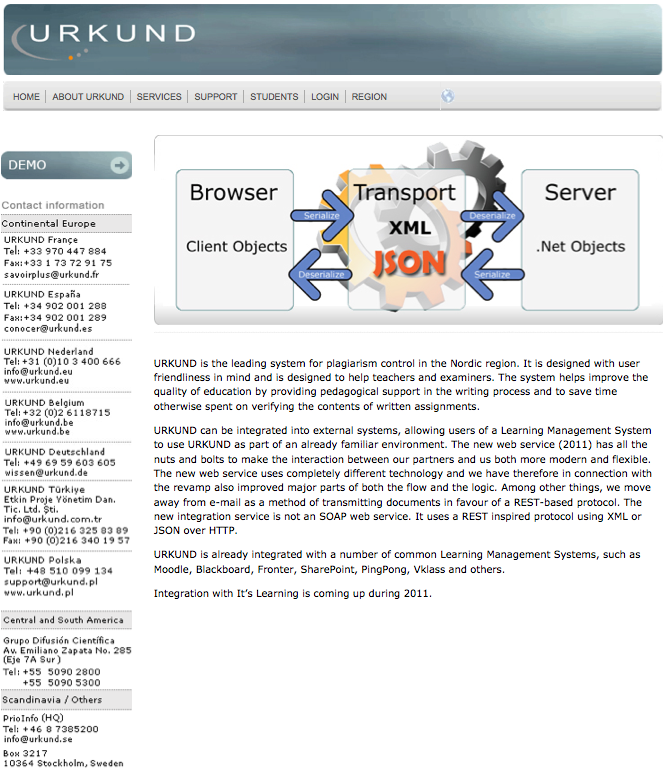
\includegraphics[width=0.97\textwidth]{images/software_systems/urkund_1.png}
  }
  \caption{Urkund Website}
  \label{fig:Urkund Website}
\end{figure}

\textbf{Business Promotion}
\begin{quote}
"URKUND was born from the academic world. A team of teachers developed the idea of a web based service that would help them detect and deter plagiarism and URKUND was born in the fall of 2000. The problem of plagiarism received much attention in the media and more and more began realise the scope of the problem and the need of a tool to support the pedagogical work. URKUND continued to grow and develop over the years and came to be recognised as Sweden's foremost anti plagiarism service.

Today, URKUND is present in our neighbouring countries and continental Europe as well as the USA, Asia and the Middle East.

URKUND is a natural part of the educational work of the academic world today. Both faculty and students are aware of the immediate and long term benefits of our system."
\end{quote}\citep{UrkundTest}

Urkund is the last system in our comparison of partially useful systems. It ranked at the 5th position in the HTW "Plagiarism Detection System Test" 2010. The company is from sweden and started their business in 2000. In this test it ranked high in effectiveness but on the other side it's not easy to use. It has problems in the translation and after the redesign 2008 the usability was going worse.
Overall "the navigation is confusing, the layout at times catastrophic with texts overlapping fields,  the printed reports could be better, the error messages are cryptic, and the link descriptions are unclear."\citep{UrkundTest}


 \begin{figure}[!h]
  \centering
  \fbox{
    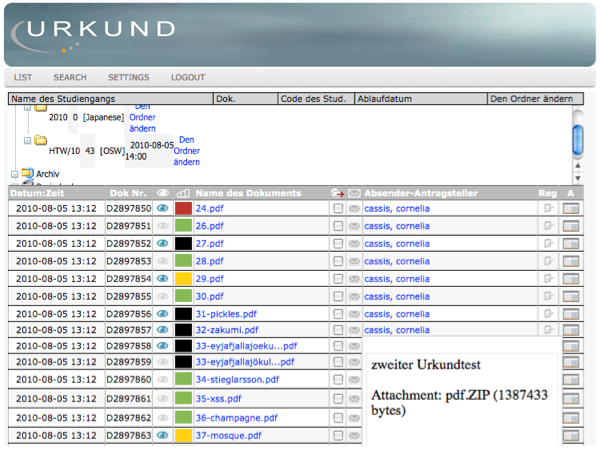
\includegraphics[width=0.97\textwidth]{images/software_systems/urkund_2.png}
  }
  \caption{Urkund List view}
  \label{fig:Urkund_list_view}
\end{figure}

 \begin{figure}[!h]
  \centering
  \fbox{
    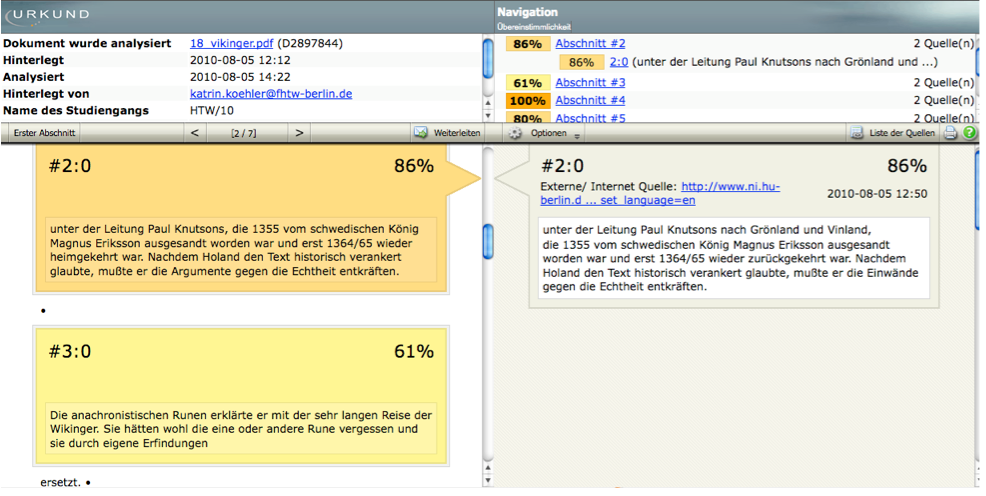
\includegraphics[width=0.97\textwidth]{images/software_systems/urkund_3.png}
  }
  \caption{Urkund Report}
  \label{fig:urkund_report}
\end{figure}

\subsubsection{Urkund costs}
Not stated.


\newpage

\subsection{Resume commercial software systems}

Although over the years there are more software detection systems that claim to check text reliable if it's plagiarism or not, but the quality of the systems decreases. 
A big problem that some of the tested systems offer "ghostwriting".

There are a quite a few differences between the benchmarking in 2008 and 2010, specially the ability to detect plagiarism in text which dropped and switched words. The best systems only reached 70\%.

The "Plagiat Team" updated the test with short essays in german, english and japanese.
Also took aspects of design, language consistency, navigation and so on.
They  categorized the systems in partially useful, barely useful, and useless for university purposes. The best systems between 60 and 70\% effectiveness were PlagAware, Turnitin, Ephorus, PlagScan and Urkund. \citep{PlagiatTeam} 

The recommendation of  the \citet{PlagiatTeam} were that the focus should be on teaching students about plagiarism and how to avoid it instead of investing time in using software. 


\section{Vroni Plag}
\textit{VroniPlag}  is a wiki platform which many volunteers, who are ready to give their free time, their money or 
their books/resources etc. work on. They collaborate with each other in order to detect plagiarism in dissertations or
habilitations.

The wiki \textit{VroniPlag} was founded in 2011 in march the 28th. \textit{VroniPlag}  is mainly reviewing dissertations, which could be plagiats. It is an developed equivalent of the \textit{GuttenPlag} wiki. The founder of VroniPlag is Martin Heidingsfelder.
\citep{Wikipedia}


VroniPlag is named after the first case which they published. The case was the one of Veronica Saß.

Because it is a wiki page, which means open to all, every one could join in. If somebody is interested in a public 
case, he can feel free to edit the page without asking for an allowance. In the chat portal of this community, one could 
ask for more help or to take a look at the list of waiting fragments.

Before starting detection, there are some information that a collaborator might know.

\subsection{Plagiarism detection steps}
A suspicious case is called \textit{candidate case}. This case is still not public for all. If a user has detected some 
suspicious part of a dissertation, he/she may first go to Chat portal to indicate his/her suspicion. He/she has 
also to give at least one original text source as proof for it. If it is well reasoned that there is an existing 
plagiarism, he/she must see if there are enough collaborators, who are ready to spend their time to work with.

The candidate case has been given an anonymous name and not public until there is proof, that there is at 
least 10\% of the pages, in which plagiarized texts are found. After that the case will be published with the 
name of the author.

During the detection process, the candidate case will be divided into smaller fragments. The fragments will be checked 
carefully if there is a plagiarism found. If there is, a report is created which shows in which fragment the 
plagiarism is found. The original source is also correspondingly given.

After checking, fragment’s state is changed to \enquote{to be proofed.} That means, this fragment must be checked again  by a 
second inspector. The result will be classified in corresponding category (see \nameref{sec:classification}).

After all fragments are checked, an overview of detected plagiarism will be generated. The overview includes the following 
parts:

\subsubsection{Part 1:} 

The whole page numbers with two different colors. The page number includes also a link redirecting to corresponding 
fragment.

\begin{itemize}
\item Grey: page in which there is no plagiarism found or not checked yet.
\item Blue: page with plagiarised texts found. The link goes to the plagiarized text in comparison with  the source as well.
\end{itemize}


\begin{figure}[!h]
  \centering
    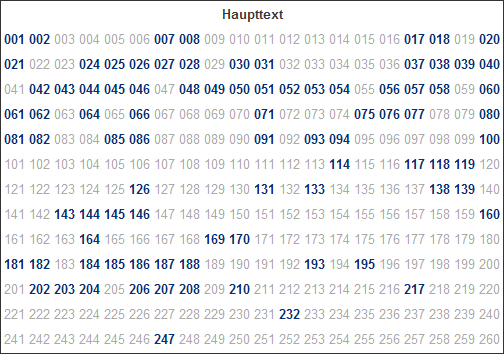
\includegraphics[width=0.95\textwidth]{images/vroni-pages.png}
  \caption{Source: \url{http://de.vroniplag.wikia.com/wiki/Lm}, 19/03/2012, 08:53}
  \label{fig:vroniPages}
\end{figure}


\subsubsection{Part 2:} 

The second part is a generated barcode label which performs the percent of plagiarism found in one page with 
different colors.

\begin{itemize}
\item Blue: pages which are not calculated in the dissertation such as Index, Appendix, literature list
\item Grey: suspiciously plagiarized
\item Black: verified that 100\% of the page is plagiarized
\item Brown: verified that more than 50\% of the page is plagiarized
\item Red: verified that more than 75\% of the page is plagiarized
\end{itemize}

\begin{figure}[!h]
  \centering
    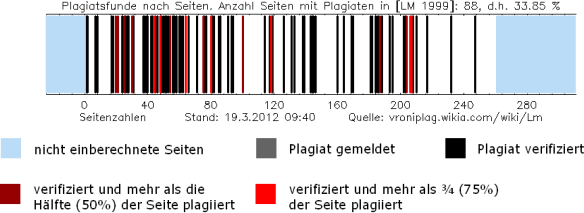
\includegraphics[width=0.95\textwidth]{images/vroni-barcode.png}
  \caption{Source: \url{http://de.vroniplag.wikia.com/wiki/Lm}, 19/03/2012, 08:54}
  \label{fig:vroniBarcode}
\end{figure}



If there is more than 10\% of the whole pages plagiarized, the case will be public on wiki. Then a report will be sent 
to the university, where the dissertation is finished.

\subsection{Technical support}

Most of the work by VroniPlag is done by hand. For example collaborators could use Google to search for sources, 
or they borrow books from the library and scan the texts. Generally there is no special software to help detect 
plagiarism, but collaborator could feel free to choose some of the existing software to help work faster.


	 \begin{figure}[!h]
  \centering
  \fbox{
    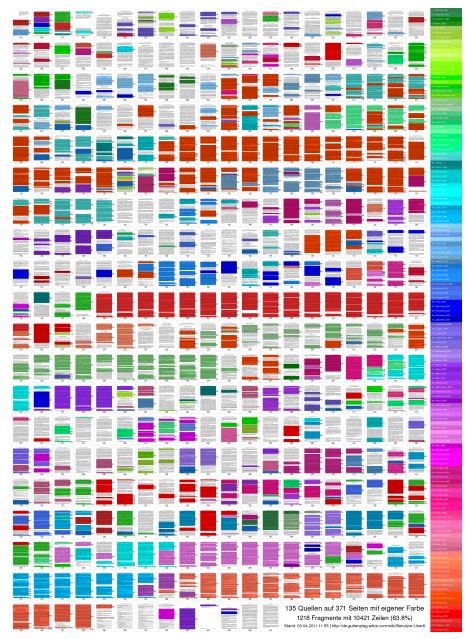
\includegraphics[width=0.6\textwidth]{images/colors.png}
  }
  \caption{colors}
  \label{fig:colors}
\end{figure}

	
